\subsection{Transcendence bases}

PROPOSITION 4. --- Let E be an extension of a field K and S and T two subsets of E. Then the following properties are equivalent :

\begin{enumerate}
\def\labelenumi{\alph{enumi})}
\item
  \(\mathbf{S} \cup \mathbf{T}\) is algebraically free over \(\mathbf{K}\) and \(\mathbf{S} \cap \mathbf{T} = \emptyset\) .
\item
  S is algebraically free over K and T is algebraically free over K(S).
\item
  T is algebraically free over K and S is algebraically free over K(T).
\end{enumerate}

Evidently it is enough to prove that \(a)\) and \(b)\) are equivalent.

\(a) \Rightarrow b)\) : Suppose that \(a)\) holds. Since S is contained in S \(\cup\) T, it is algebraically free over K. If T is not algebraically free over K(S), there exists (Prop. 3) a finite family \((y_j)_{1 \leq j \leq n}\) of distinct elements of T which is algebraically related over K(S). Hence there is a non-zero polynomial \(f\) in the ring K(S) {[}Y \(_1\) , \ldots, Y \(_n\) {]} such that \(f(y_1, ..., y_n) = 0\) ; after multiplying \(f\) if necessary by a non-zero element of K{[}S{]} we may suppose that all the coefficients of \(f\) belong to K{[}S{]}. The coefficients of \(f\) are polynomials in a finite number of distinct elements \(x_i\) ( \(1 \leq i \leq m\) ) of S, with coefficients in K. The elements \(x_1, ..., x_m\) , \(y_1, ..., y_n\) are pairwise distinct because S \(\cap\) T = ∅. The relation \(f(y_1, ..., y_n) = 0\) may thus be written

\[
g \left(x _ {1}, \dots , x _ {m}; y _ {1}, \dots , y _ {n}\right) = 0,
\]

where \(g\) is a non-zero polynomial of \(\mathbf{K}[\mathbf{X}_1, \ldots, \mathbf{X}_m, \mathbf{Y}_1, \ldots, \mathbf{Y}_n]\) , and such a relation contradicts the hypothesis that \(\mathbf{S} \cup \mathbf{T}\) is algebraically free.

\(b) \Rightarrow a)\) : Suppose that \(b)\) holds. In the first place it is clear that \(\mathrm{T} \cap \mathrm{K}(\mathrm{S}) = \emptyset\) and \(a\) fortiori \(\mathrm{S} \cap \mathrm{T} = \emptyset\) . It suffices to show that if \(x_i\) ( \(1 \leqslant i \leqslant m\) ) are distinct elements of \(\mathrm{S}\) , finite in number, and \(y_j\) ( \(1 \leqslant j \leqslant n\) ) distinct elements of \(\mathrm{T}\) finite in number, then the set of the \(x_i\) and \(y_j\) is algebraically free over \(\mathrm{K}\) (Prop. 3). Consider a polynomial \(f \in \mathrm{K}[\mathrm{X}_1, \ldots, \mathrm{X}_m, \mathrm{Y}_1, \ldots, \mathrm{Y}_n]\) such that \(f(x_1, \ldots, x_m, y_1, \ldots, y_n) = 0\) and put \(f = \sum_{\alpha_1 \ldots \alpha_n} \varphi_\alpha \mathrm{Y}_1^{\alpha_1} \ldots \mathrm{Y}_n^{\alpha_n}\) with \(\varphi_\alpha \in \mathrm{K}[\mathrm{X}_1, \ldots, \mathrm{X}_m]\) for all

\(\alpha = (\alpha_{1}, \ldots, \alpha_{n}) \in \mathbf{N}^{n}\) . Let \(g = f(x_{1}, \ldots, x_{m}, \mathbf{Y}_{1}, \ldots, \mathbf{Y}_{n})\) ; then \(g\) is a polynomial in the ring \(\mathbf{K}[\mathbf{S}][\mathbf{Y}_{1}, \ldots, \mathbf{Y}_{n}]\) and the relation \(f(x_{1}, \ldots, x_{m}, y_{1}, \ldots, y_{n}) = 0\) may be written \(g(y_{1}, \ldots, y_{n}) = 0\) . Since \(T\) is algebraically free over \(\mathbf{K}(\mathbf{S})\) , each of the coefficients \(\varphi_{\alpha}(x_{1}, \ldots, x_{m})\) of \(g\) is zero; since \(S\) is algebraically free over \(K\) , we have \(\varphi_{\alpha} = 0\) for all \(\alpha \in \mathbf{N}^{n}\) , and hence \(f = 0\) .

COROLLARY. --- Let E be an extension of a field K and S a subset of E which is algebraically free over K. If \(x \in E\) is transcendental over \(\mathrm{K}(\mathrm{S})\) , then \(S \cup \{x\}\) is algebraically free over K.

PROPOSITION 5. --- Let E be an extension of the field K. For a subset S of E to be algebraically free over K it is necessary and sufficient that for each \(x \in S\) , the element x should be transcendental over the field \(\mathrm{K}(\mathrm{S} - \{x\})\) .

The condition is necessary by Prop. 4.

To prove the sufficiency it is enough (Prop. 3) to show that every finite sequence \((x_{1},\ldots,x_{n})\) of distinct elements of S is algebraically free. Now by hypothesis \(x_{i}\) is transcendental over \(\mathrm{K}(x_{1},\ldots,x_{i-1})\) for \(1\leqslant i\leqslant n\) , and now our assertion follows by induction on n from the Cor. to Prop. 4.

PROPOSITION 6. --- Let E be an extension of a field K and X an algebraically free subset of E over K. If \(K' \subset E\) is an algebraic extension of K then X is algebraically free over \(K'\) .

Arguing by contradiction, let us suppose that X is algebraically related over \(K'\) . By Prop. 5 there exists an element \(x \in X\) which is algebraic over the field \(\mathbf{K}'(\mathbf{M})\) , where \(\mathbf{M} = \mathbf{X} - \{x\}\) . Since \(\mathbf{K}'(\mathbf{M}) = \mathbf{K}(\mathbf{M})(\mathbf{K}')\) and \(K'\) is algebraic over K, Cor. 2 of V, p.~18 shows that \(\mathbf{K}'(\mathbf{M})\) is algebraic over \(\mathbf{K}(\mathbf{M})\) ; since x is algebraic over \(\mathbf{K}'(\mathbf{M})\) , it is therefore algebraic over \(\mathbf{K}(\mathbf{M}) = \mathbf{K}(\mathbf{X} - \{x\})\) , by Prop. 3 of V, p.~19. Now Prop. 5 shows X to be algebraically related over K and we have a contradiction.

DEFINITION 3. --- A subset B of an extension E of a field K is a transcendence basis of E (over K) if B is algebraically free over K and E is algebraic over K(B).

\pandocbounded{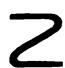
\includegraphics[keepaspectratio]{images/part002_88480e13.jpg}}

Example. --- A pure basis is a transcendence basis. On the other hand, if E is a pure extension of K, a transcendence basis of E over K is not always a pure basis of E. For example, in \(\mathbf{K}(\mathbf{X})\) , \(\{\mathbf{X}^{2}\}\) is a transcendence basis but does not generate \(\mathbf{K}(\mathbf{X})\) .

PROPOSITION 7. --- Let E be an extension of a field K. Every transcendence basis of E is a maximal element of the set (ordered by inclusion) of subsets of E algebraically free over K. Conversely, if S is a subset of E such that E is algebraic over K(S), every maximal algebraically free subset of S is a transcendence basis of E.

Let B be a transcendence basis of E over K and \(x \in E - B\) . Then x is algebraic over \(\mathrm{K}(\mathrm{B})\) ; by V, p.~107, Prop. 4, the subset \(B \cup \{x\}\) of E is not algebraically free over K, whence the first part of the proposition. Secondly, if E is algebraic over \(\mathrm{K}(\mathrm{S})\) and B is a maximal algebraically free part of S, it follows from the Cor. of Prop. 4 that every \(x \in S\) is algebraic over \(\mathrm{K}(\mathrm{B})\) ; hence (V, p.~18, Cor. 1) \(\mathrm{K}(\mathrm{S})\) is algebraic over \(\mathrm{K}(\mathrm{B})\) , and so (V, p.~19, Prop. 3), E is algebraic over \(\mathrm{K}(\mathrm{B})\) .

THEOREM 1 (Steinitz). --- Every extension E of a field K admits a transcendence basis over K. In other words, every extension of a field K is an algebraic extension of a pure extension of K.

\pandocbounded{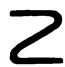
\includegraphics[keepaspectratio]{images/part002_71d10db7.jpg}}

By contrast, an extension is not always a pure extension of an algebraic extension (V, p.~171, Ex. 2).

This theorem is a consequence of the following more precise result:

THEOREM 2. --- Let E be an extension of a field K, S a subset of E such that E is algebraic over K(S) and T a subset of S which is algebraically free over K; then there exists a transcendence basis B of E over K such that \(T \subset B \subset S\) .

For the set of algebraically free subsets of S, ordered by inclusion, is a set of finite character (E, III, p.~34) by Prop. 3. By Th. 1 of E, III, p.~35 it has a maximal element B containing T, and B is a transcendence basis of E over K, by Prop. 7.

COROLLARY (« Exchange Theorem »). --- Let E be an extension of K, S a subset of E such that E is algebraic over K(S), T a subset of E which is algebraically free over K; then there exists a subset S' of S such that T ∪ S' is a transcendence basis of E over K and T ∩ S' = ∅.

For E is algebraic over \(\mathbf{K}(\mathbf{T} \cup \mathbf{S})\) and we have \(T \subset T \cup S\) .

